\documentclass{beamer}

\usepackage[utf8]{inputenc}
\usepackage{amsmath,amsfonts,amssymb}
\usepackage{url}
\usepackage{listings}
\usepackage{color}
\usepackage{moresize}
\usepackage{algorithm}
\usepackage[noend]{algpseudocode}
\usepackage{graphicx} % Allows including images
\usepackage{booktabs} % Allows the use of \toprule, \midrule and \bottomrule in tables

\definecolor{MyDarkMagenta}{rgb}{ 0.5, 0.0, 0.5 }
\definecolor{MyDarkBlue}{rgb}{ 0.0, 0.0, 0.5 }
\definecolor{MyDarkRed}{rgb}{ 0.5, 0.0, 0.0}
\definecolor{MyDarkOrange}{rgb}{0.667, 0.267, 0.0}
\definecolor{MyGray}{rgb}{0.6,0.6,0.6}

\let\oldfootnotesize\footnotesize
\renewcommand*{\footnotesize}{\oldfootnotesize\tiny}

\usetheme{Madrid}
\useinnertheme{circles}
\usecolortheme{dolphin}
\setbeamercovered{transparent}
\beamertemplatenavigationsymbolsempty
\usefonttheme{professionalfonts}

\title[SixTrackLib]{Optimising and Extending a Single-Particle Tracking Library for High Parallel Performance} % The short title appears at the bottom of every slide, the full title is only on the title page

\author[Schwinzerl et al]{M. Schwinzerl, R. De Maria, K. Paraschou, H. Bartosik, G. Iadarola, A. Oeftiger
\institute[CERN, GSI]{CERN, GSI} % Your institution as it will appear on the bottom of every slide,
}
\date{May 2021} % Date, can be changed to a custom date


\begin{document}

\begin{frame}
\begin{figure}
 \centering
 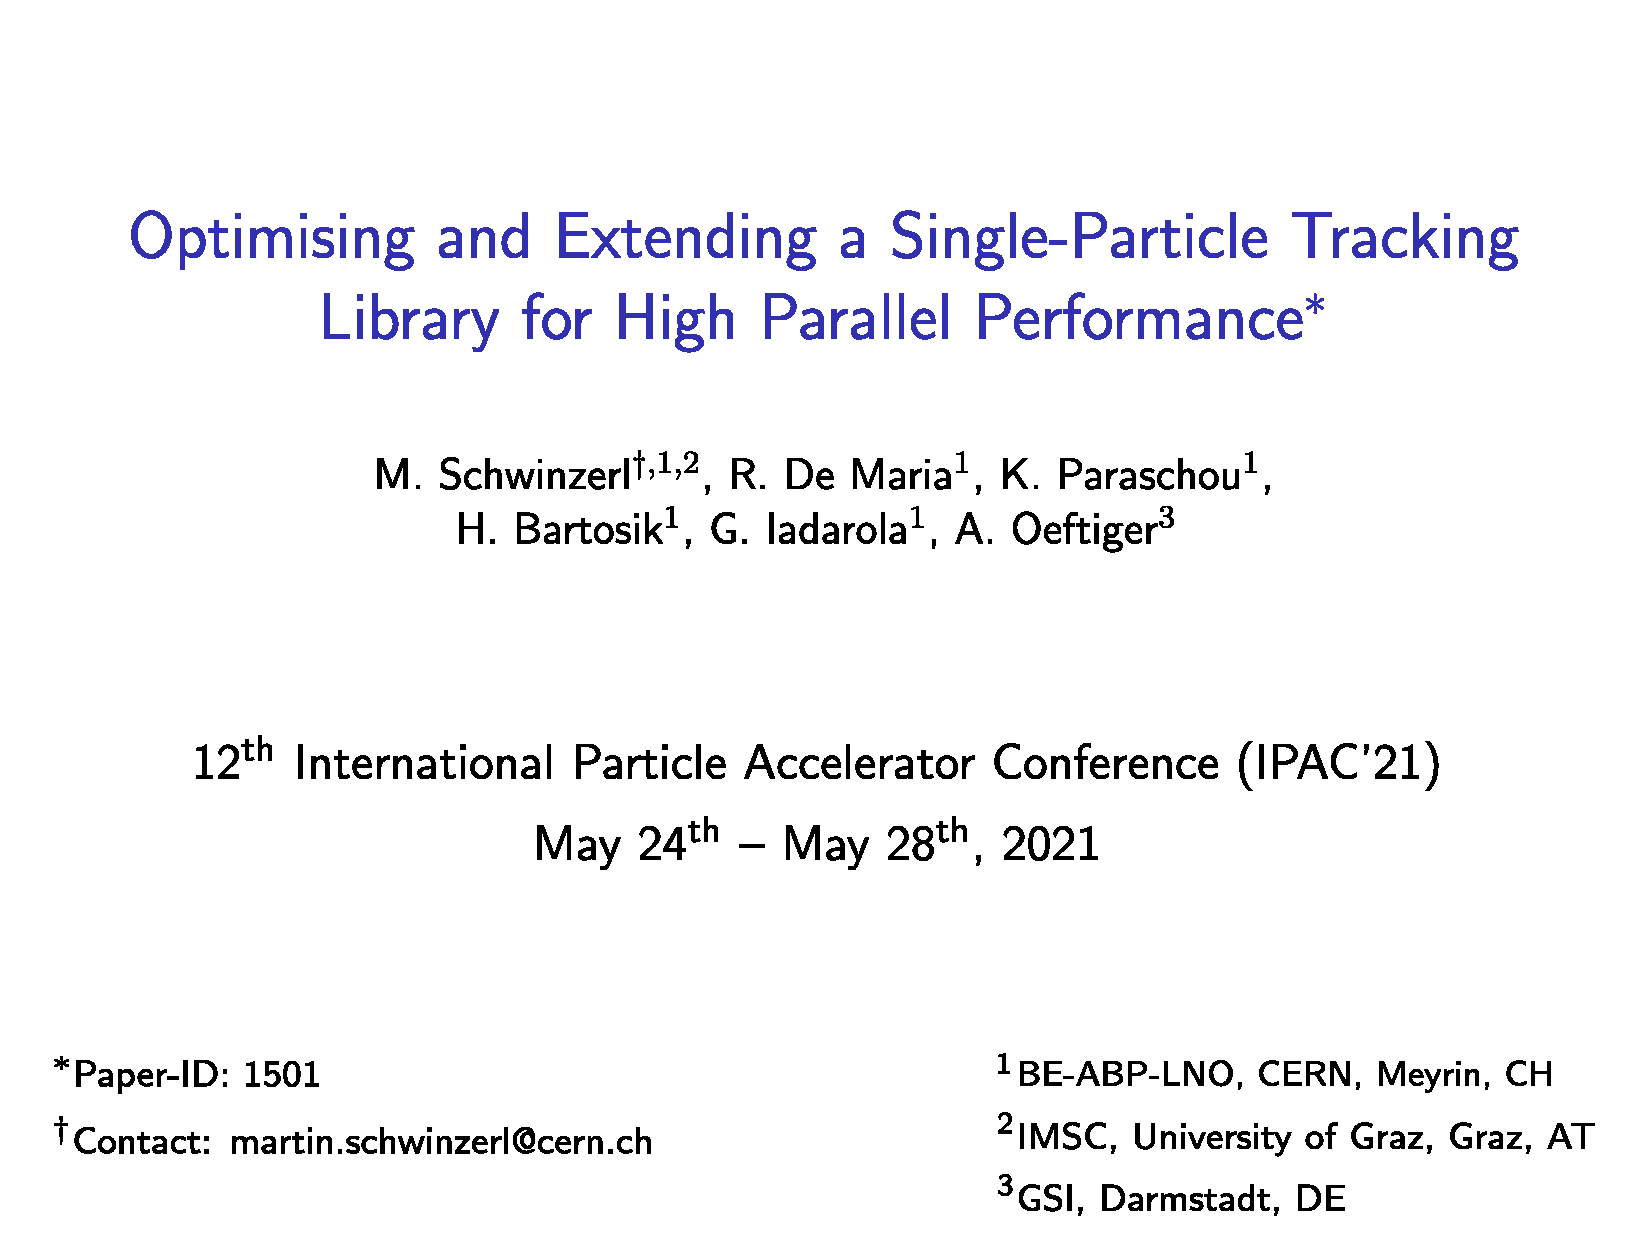
\includegraphics[width=0.95\textwidth]{poster_images/fig_title}
\end{figure}
\end{frame}

\begin{frame}
\frametitle{Introduction}
\begin{itemize}
    \item<1-> \texttt{SixTrackLib} is a {\color{MyDarkBlue} single-particle} tracking library
    \item<1-> Re-implementation of the core \texttt{SixTrack} tracking component
    \item<1-> Embeddable, minimal, usable on single CPU cores \& parallel hardware, multiple computing back-ends, common implementation of physics, high performance
\end{itemize}
\only<1>
{
    \begin{figure}[h]
        \centering
        
\includegraphics[width=0.95\textwidth]{presentation_images/fig_coordinates_00}
    \end{figure}
}
\only<2>
{
    \begin{figure}[h]
        \centering
        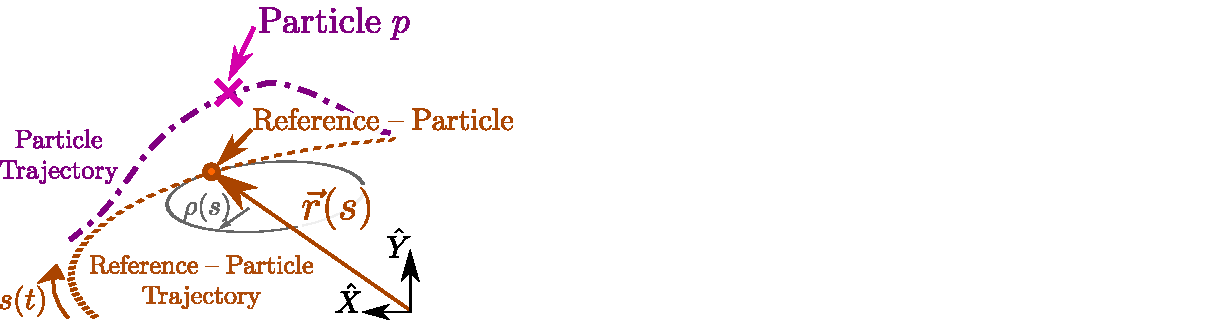
\includegraphics[width=0.95\textwidth]{presentation_images/fig_coordinates_01}
    \end{figure}
}
\only<3>
{
    \begin{figure}[h]
        \centering
        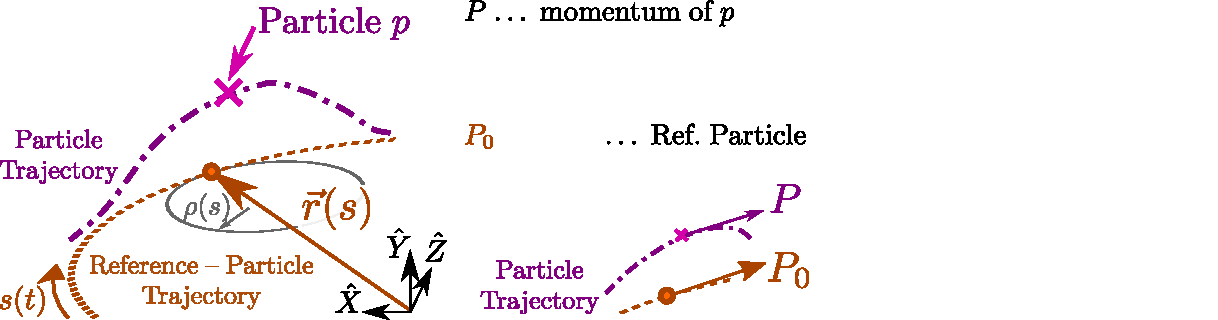
\includegraphics[width=0.95\textwidth]{presentation_images/fig_coordinates_02}
    \end{figure}
}
\only<4>
{
    \begin{figure}[h]
        \centering
        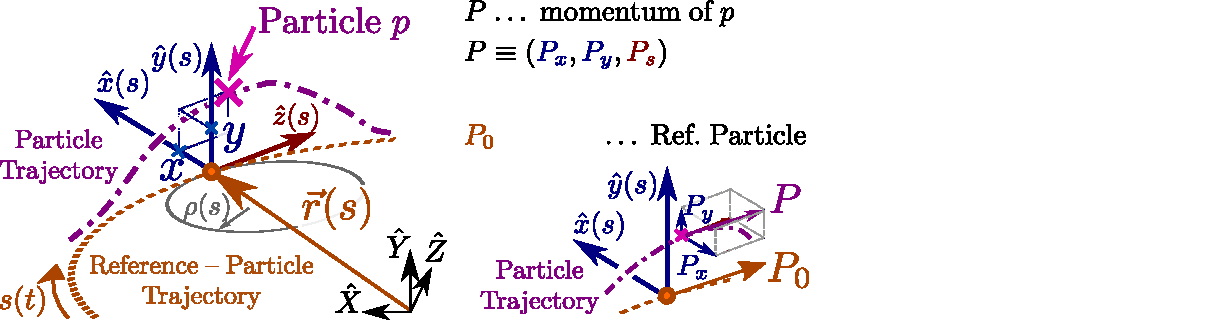
\includegraphics[width=0.95\textwidth]{presentation_images/fig_coordinates_03}
    \end{figure}
}
\only<5>
{
    \begin{figure}[h]
        \centering
        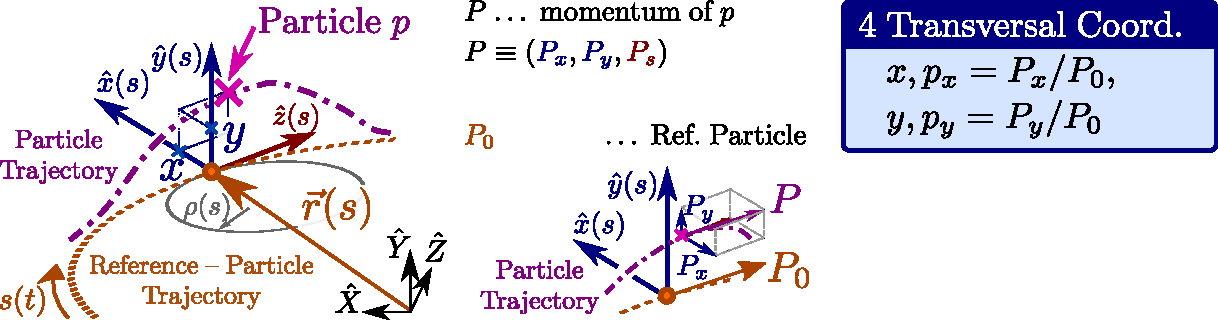
\includegraphics[width=0.95\textwidth]{presentation_images/fig_coordinates_04}
    \end{figure}
}
\only<6>
{
    \begin{figure}[h]
        \centering
        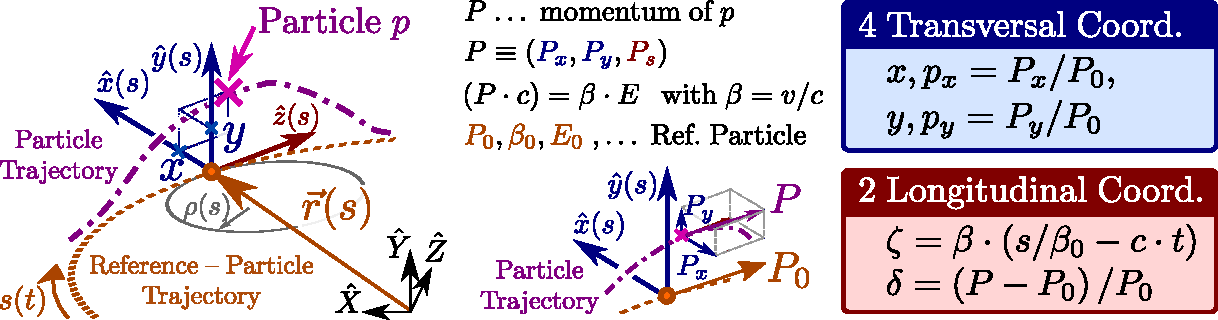
\includegraphics[width=0.95\textwidth]{presentation_images/fig_coordinates_05}
    \end{figure}
}
\begin{itemize}
    \item<4-> Coordinates expressed relative to a {\color{MyDarkOrange}Reference Particle}
    \item<6-> Particle $p \equiv p\left( x, p_x, y, p_y, \zeta, \delta\right)$ in $6D$ phase-space
\end{itemize}
\end{frame}


\begin{frame}[t]
\frametitle{Implementation - Tracking Algorithm}
\begin{itemize}
 \item<1-> Accelerator $\leadsto$ Sequence of idealised {\color{MyDarkBlue}``beam elements''} ({\color{MyDarkBlue}Lattice})
 \item<2-> {\color{MyDarkBlue}Map:} describes the effect of a beam element $E_i$ on particle $p$
 \item<3-> $p\left( i \right) \gets E_i\left( p\left( i - 1 \right) \right)${\only<4->{\color{MyDarkRed} $\;\;\Longrightarrow$ inherently sequential!}}
 \item<5-> For single particle $(N_p = 1) \rightarrow$ very limited parallelism in some $E_i$
\end{itemize}

\begin{columns}
\begin{column}{0.6\textwidth}
\begin{itemize}
 \item<6-> For $N_p > 1$: $p_j$ and $p_k$ do not interact (single-particle!)
 \item<7-> $\Rightarrow$ {\color{MyDarkBlue}Embarrisingly parallel problem}
 \item<8-> {\color{MyDarkRed}Baseline Implementation:}
    \begin{itemize}
        \item<8->Vectorised sequential (CPU)\&\newline parallel (\texttt{OpenCL}, \texttt{CUDA}) back-ends
        \item<9->Lattice: \texttt{global} memory
        \item<9->Particles: \texttt{struct-of-arrays}, \texttt{global} memory
    \end{itemize}
 \item<3-> {\color{MyDarkBlue}Note:} particles can get ``{\color{MyDarkRed}lost}'' $\rightarrow$ stop applying subsequent $E_i$
\end{itemize}
\end{column}
\begin{column}{0.35\textwidth}
\only<1>
{
    \begin{figure}[H]
        \centering
        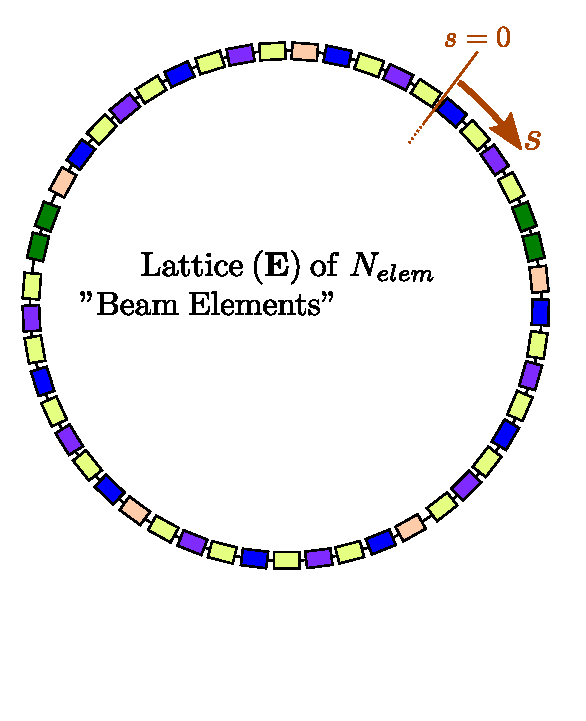
\includegraphics[width=\textwidth]{presentation_images/fig_tracking_algorithm_01}
    \end{figure}
}
\only<2>
{
    \begin{figure}[H]
        \centering
        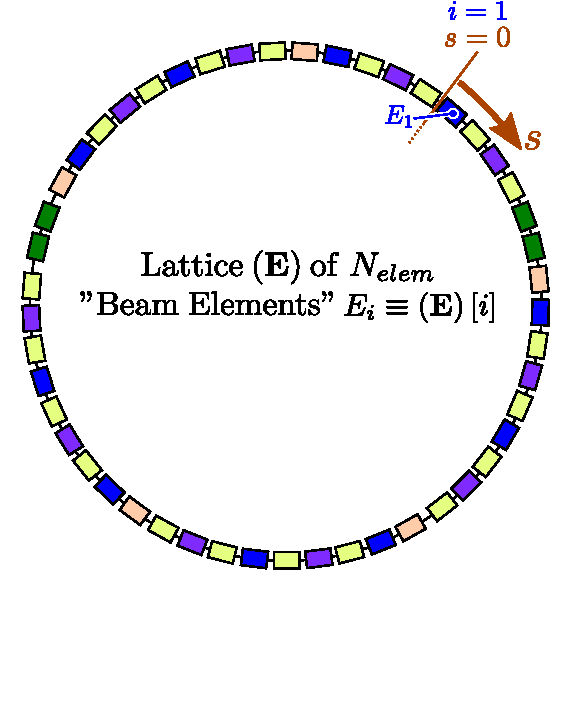
\includegraphics[width=\textwidth]{presentation_images/fig_tracking_algorithm_02}
    \end{figure}
}
\only<3>
{
    \begin{figure}[H]
        \centering
        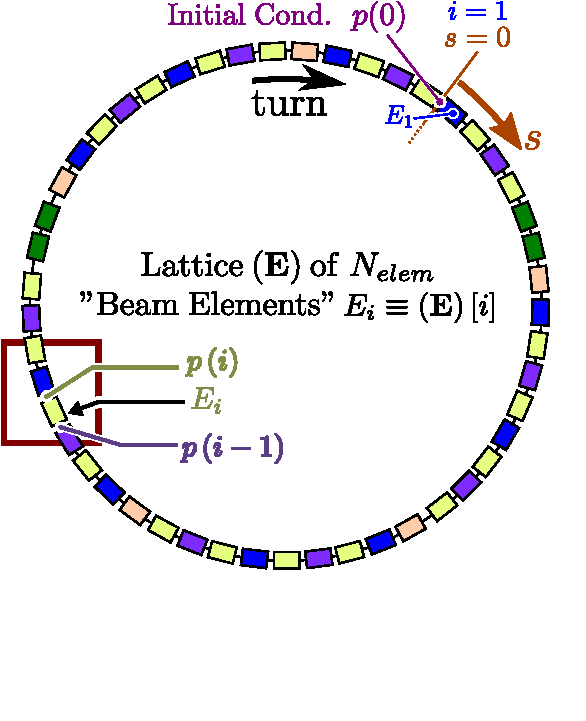
\includegraphics[width=\textwidth]{presentation_images/fig_tracking_algorithm_03}
    \end{figure}
}
\only<4->
{
    \begin{figure}[H]
        \centering
        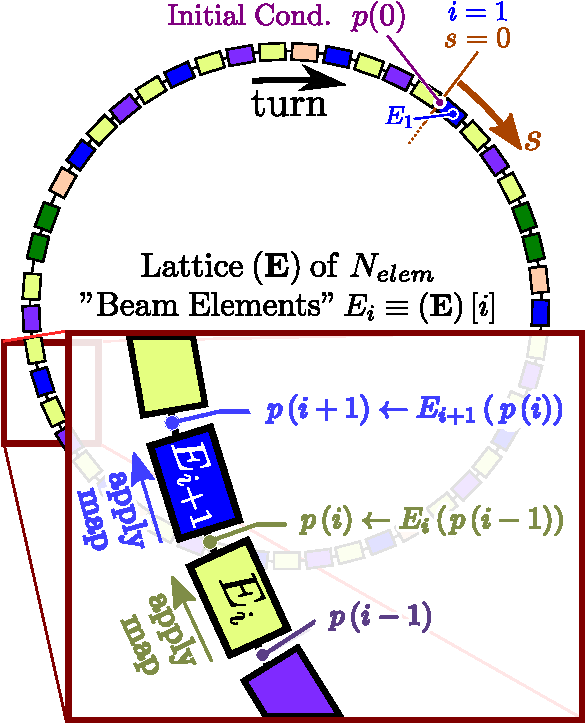
\includegraphics[width=\textwidth]{presentation_images/fig_tracking_algorithm_04}
    \end{figure}
}
\end{column}
\end{columns}
\end{frame}

\begin{frame}
    \frametitle{Baseline Performance}
    \begin{itemize}
        \item<1->LHC lattice (with imperfections, no beam-beam/space charge), $N_p: 10^0$ to $10^6$ particles, $(P_0 \cdot c) = 6.5\;\text{TeV}$, no lost particles.
        \item<2->{\color{MyDarkBlue}Normalised tracking time\footnote{$N \ldots$ number of turns. Especially for small
                  $N_p$, a larger number of turns (i.e. $100 - 1000$) has to be tracked to get reliable timings.
                  Normalising by both $N_p$ and $N$ allows a comparison across several orders of magnitude.}:} $t_{track} = t_{elapsed}/\left( N_p \cdot N \right)$ (less is better)
    \end{itemize}
    \only<1-2>
    {
        \begin{figure}[H]
            \centering
            
\includegraphics[width=0.65\textwidth]{presentation_images/baseline_benchmark_overview_00}
        \end{figure}
    }
    \only<3>
    {
        \begin{figure}[H]
            \centering
            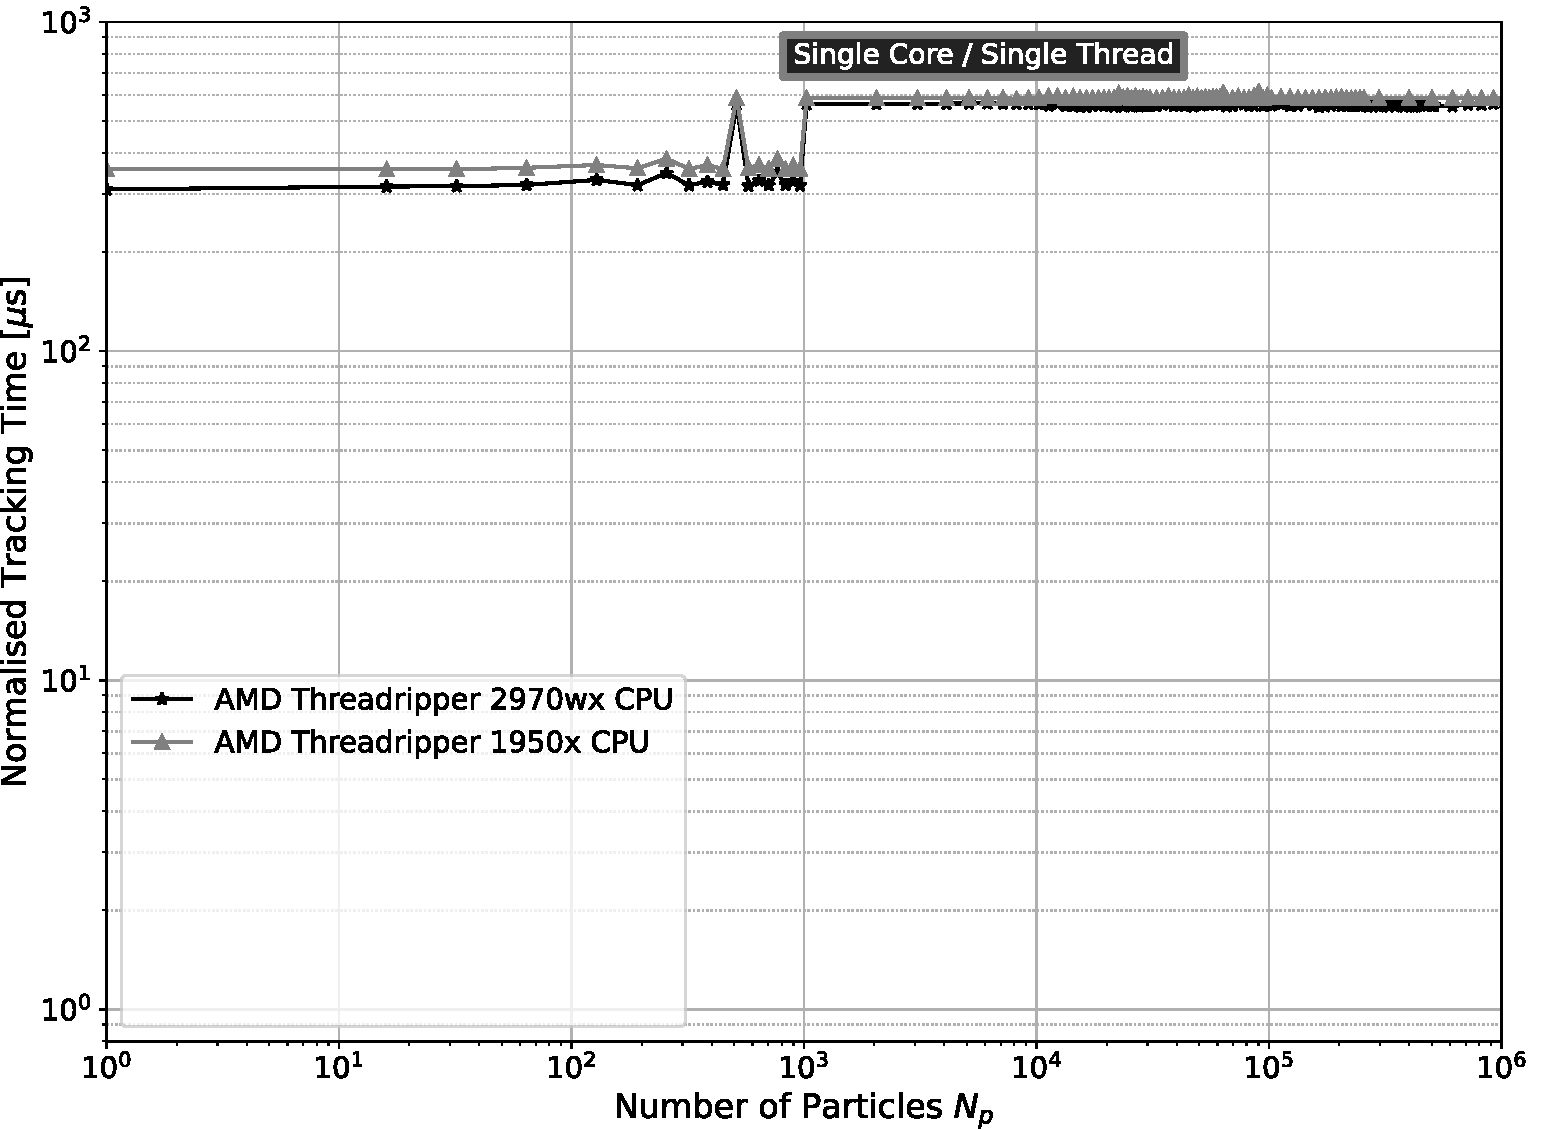
\includegraphics[width=0.65\textwidth]{presentation_images/baseline_benchmark_overview_01}
        \end{figure}
    }
    \only<4>
    {
        \begin{figure}[H]
            \centering
            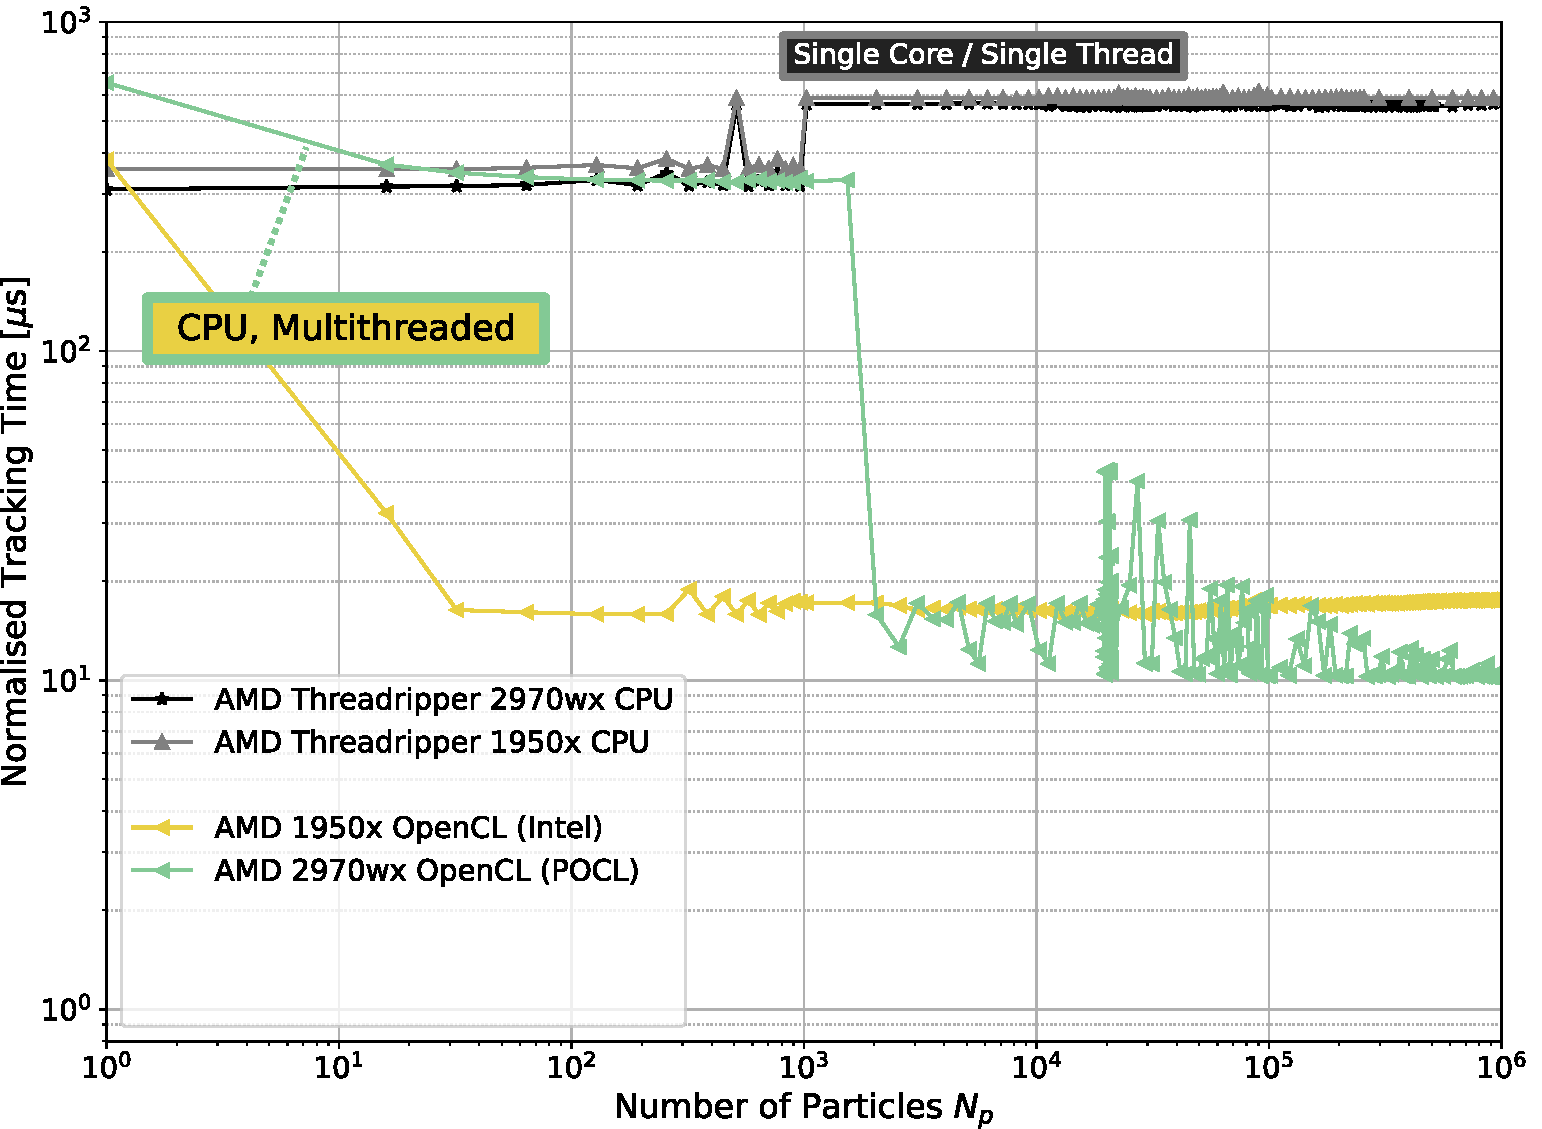
\includegraphics[width=0.65\textwidth]{presentation_images/baseline_benchmark_overview_02}
        \end{figure}
    }
    \only<5>
    {
        \begin{figure}[H]
            \centering
            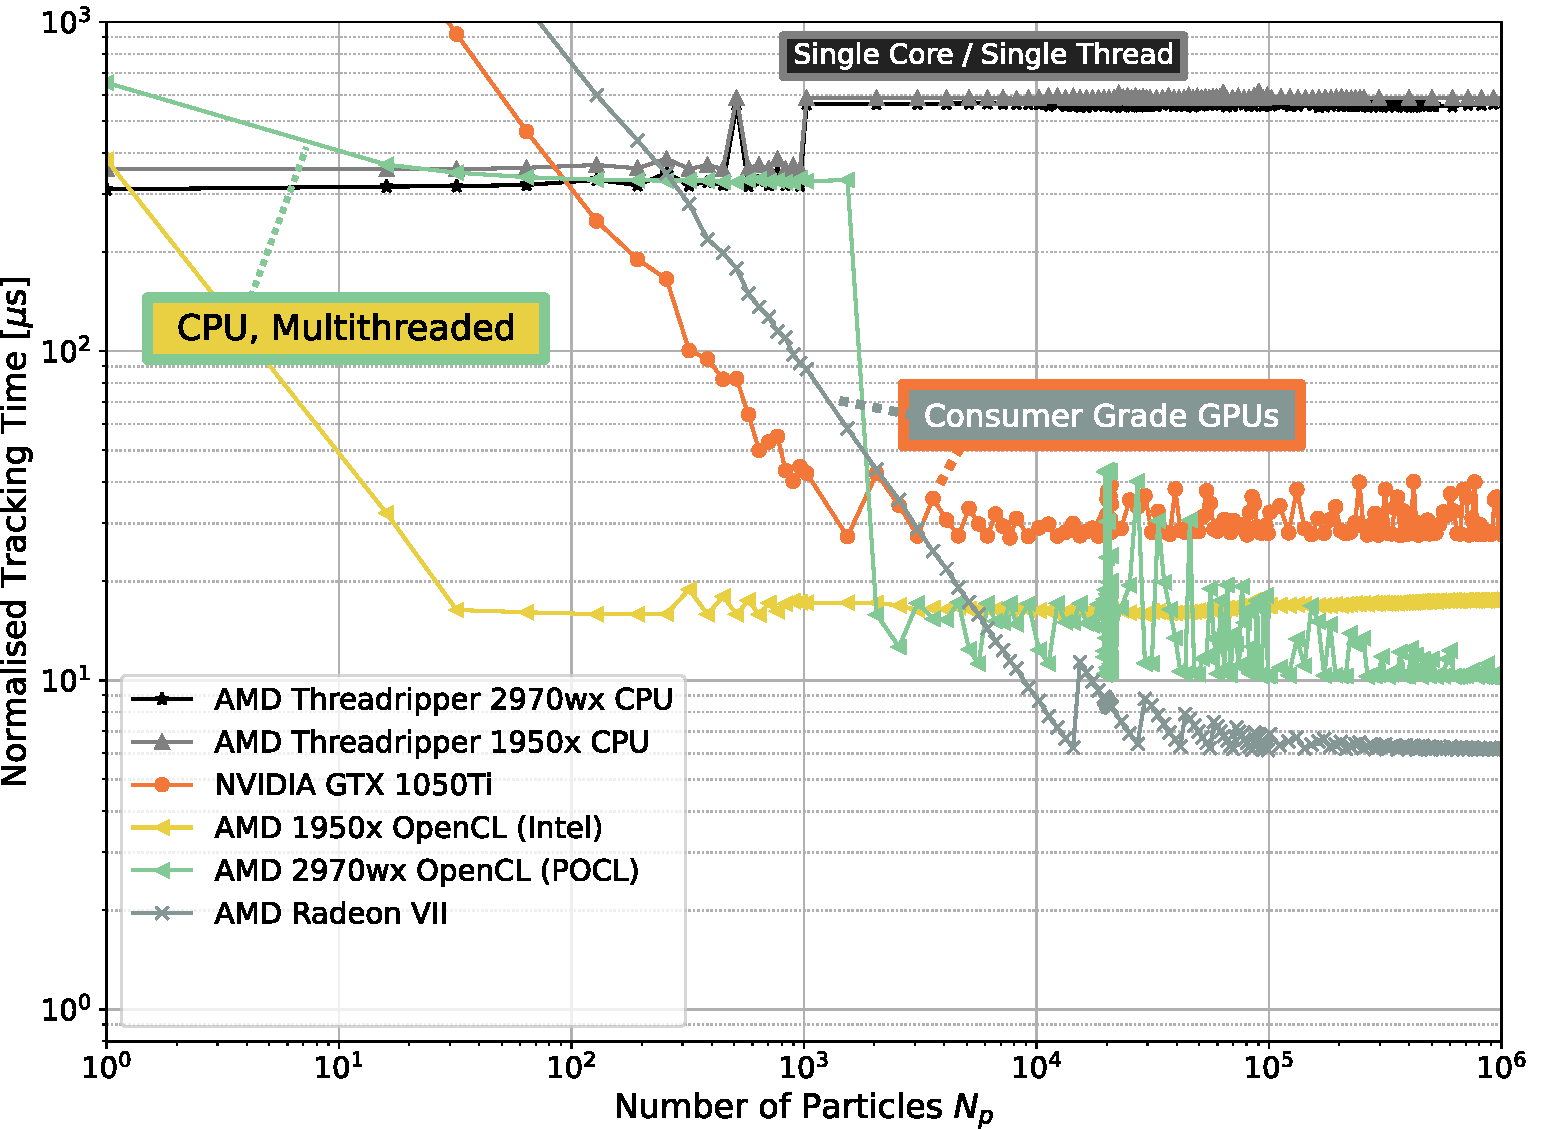
\includegraphics[width=0.65\textwidth]{presentation_images/baseline_benchmark_overview_03}
        \end{figure}
    }
    \only<6>
    {
        \begin{figure}[H]
            \centering
            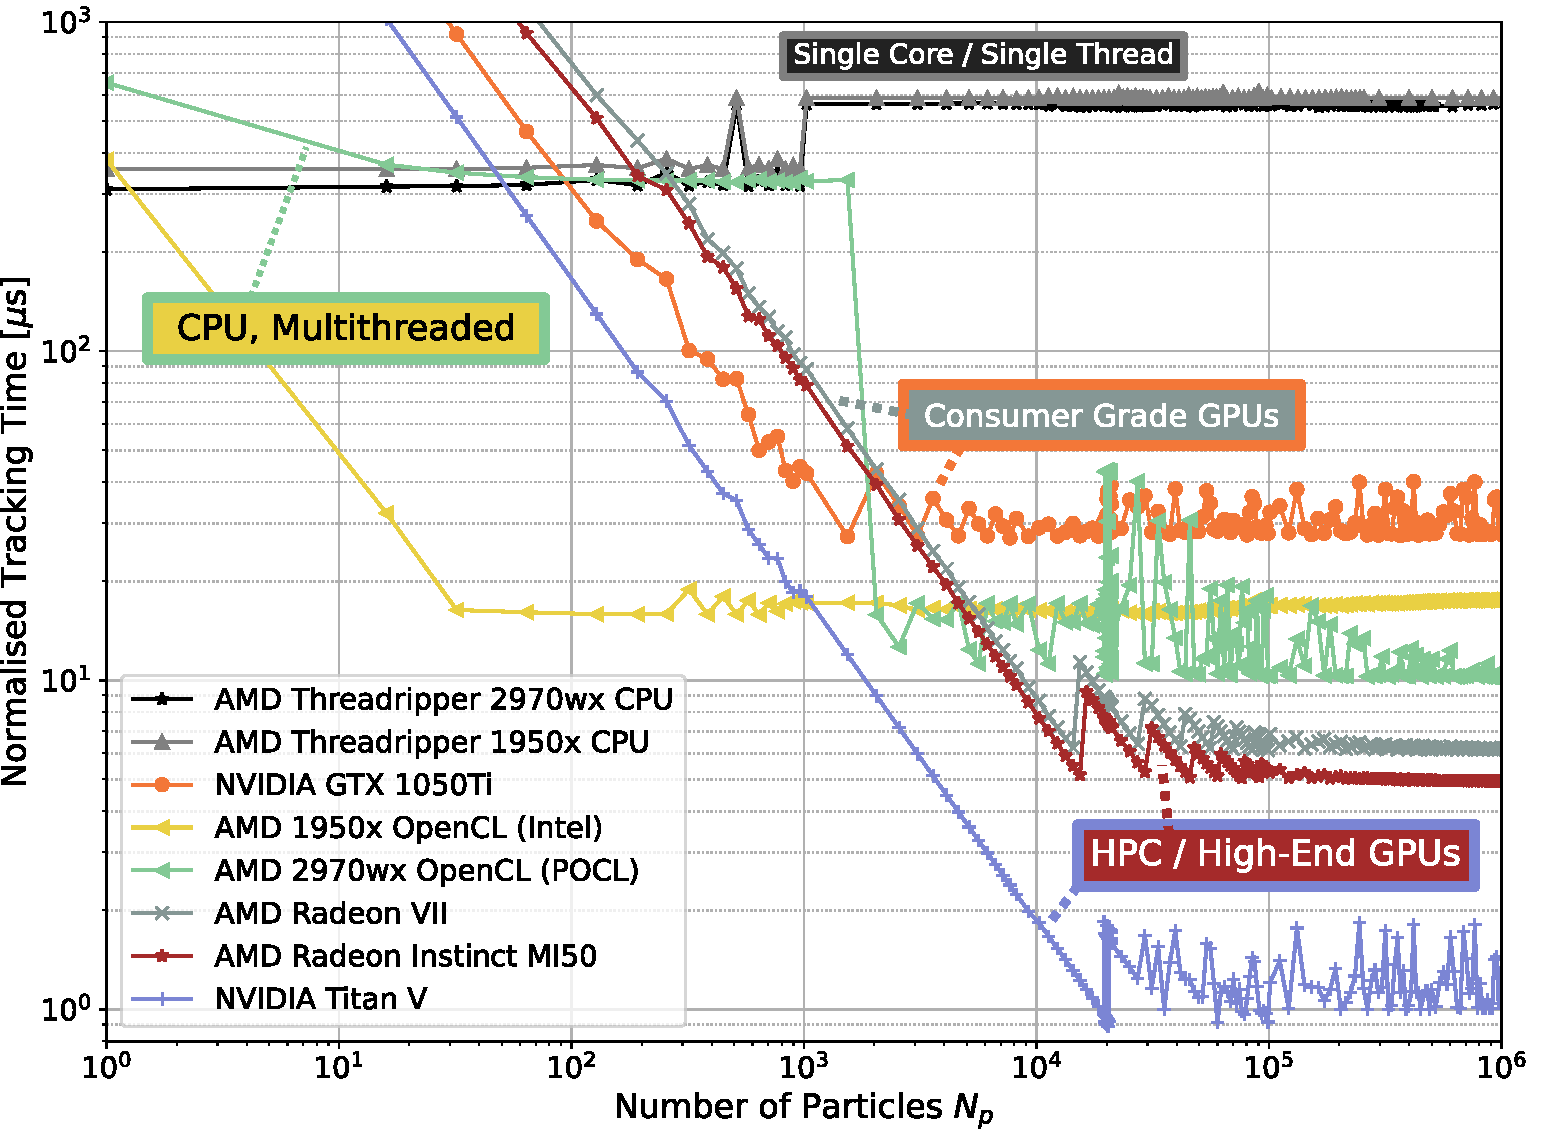
\includegraphics[width=0.65\textwidth]{presentation_images/baseline_benchmark_overview_04}
        \end{figure}
    }
    \only<7>
    {
        \begin{figure}[H]
            \centering
            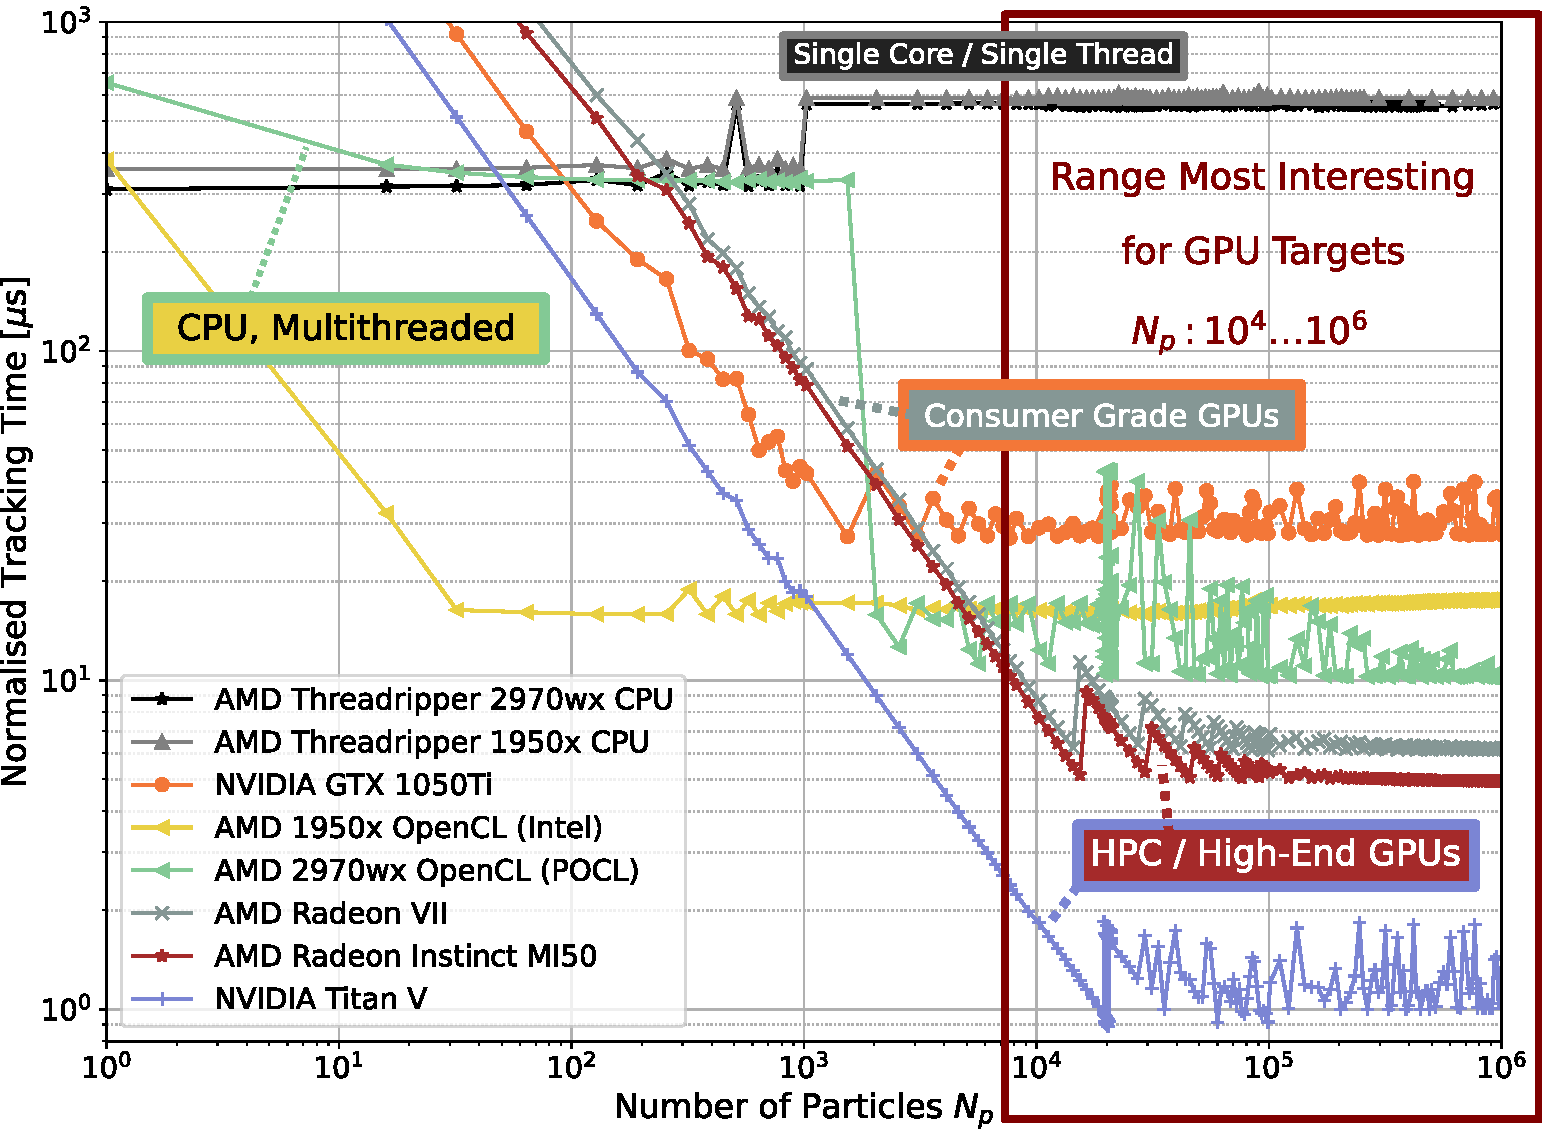
\includegraphics[width=0.65\textwidth]{presentation_images/baseline_benchmark_overview_05}
        \end{figure}
    }
    \only<8>
    {
        \begin{figure}[H]
            \centering
            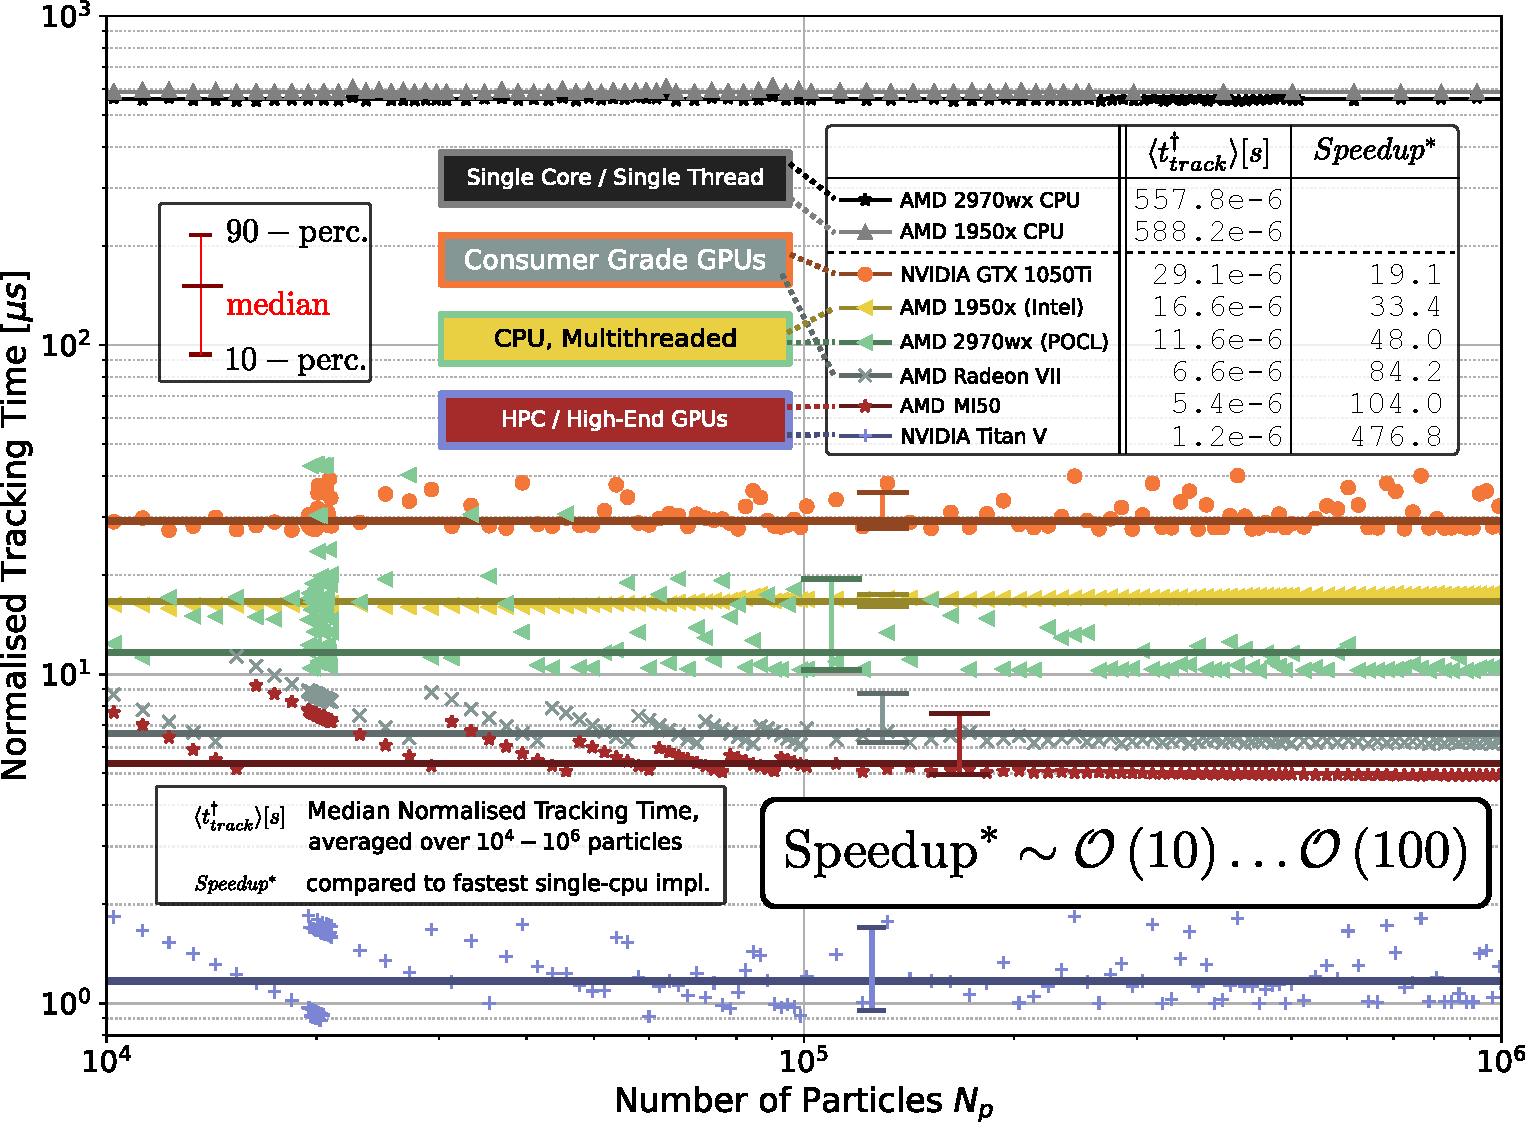
\includegraphics[width=0.65\textwidth]{presentation_images/fig_benchmark_baseline_detail}
        \end{figure}
    }
\end{frame}

\begin{frame}
    \frametitle{Optimisation}
    \begin{itemize}
        \item Attempt optimisation by a) changing memory model of particles, b) simplifying tracking logic, and c) optimise resource
        usage within maps
        \item {\color{MyDarkRed}Improvement} by factors approaching $1.5$ to $2.0\times$ for $N_p > 10^4$
    \end{itemize}
    \begin{figure}[H]
        \centering
        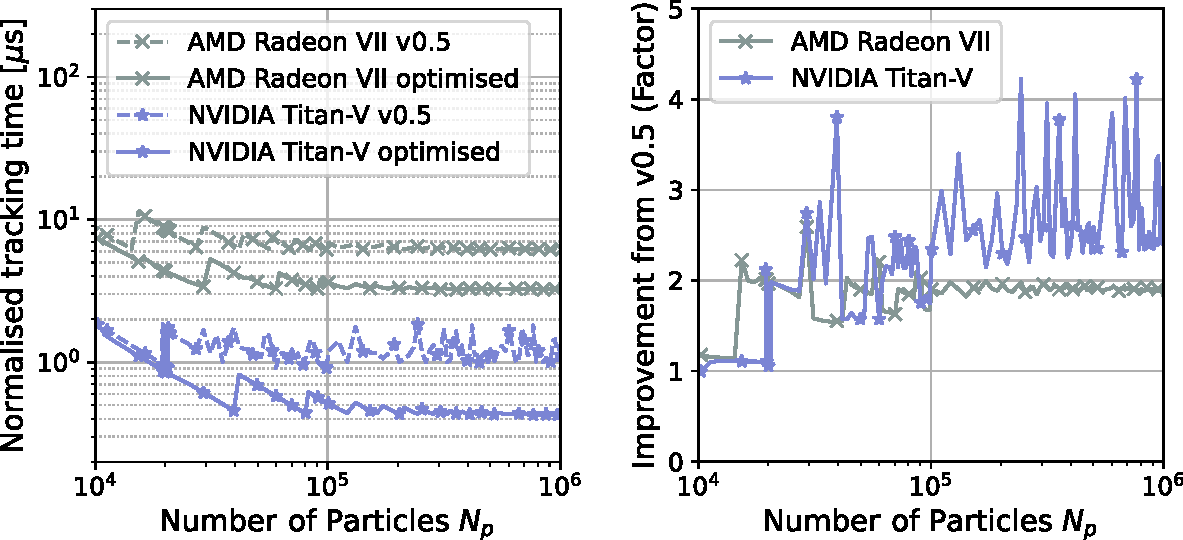
\includegraphics[width=0.85\textwidth]{presentation_images/fig_performance_optimisation}
    \end{figure}
\end{frame}

\begin{frame}
    \frametitle{Conclusions \& Outlook}
    \begin{itemize}
     \item Implementing a tracking library with multiple backends and high performance across a wide range of $N_p$ is feasible
     \item \texttt{SixTrackLib}'s baseline performance is already quite suitable for a wide range of applications
     \item Optimisations can give significant increases in performance
     \item However, further investigations about effects contributing to and limiting the scalability and trade-offs for the optimisations are required
    \end{itemize}
\end{frame}

\begin{frame}
    \begin{center}
    {\HUGE\usebeamerfont*{frametitle}\usebeamercolor[fg]{frametitle}Thank You For Your Attention}\\[1em]
    $\longrightarrow$ \url{https://github.com/sixtrack/sixtracklib}
    \end{center}
\end{frame}




\end{document}
